\documentclass[dvipdfmx]{jsarticle}
\setcounter{section}{2}
\setcounter{subsection}{2}
\usepackage{xr}
\externaldocument{1.2.1}
\externaldocument{1.2.2}
\usepackage{amsmath,amsfonts,amssymb,array,comment,mathtools,url,docmute}
\usepackage{longtable,booktabs,dcolumn,tabularx,mathtools,multirow,colortbl,xcolor}
\usepackage[dvipdfmx]{graphics}
\usepackage{bmpsize}
\usepackage{amsthm}
\usepackage{enumitem}
\setlistdepth{20}
\renewlist{itemize}{itemize}{20}
\setlist[itemize]{label=•}
\renewlist{enumerate}{enumerate}{20}
\setlist[enumerate]{label=\arabic*.}
\setcounter{MaxMatrixCols}{20}
\setcounter{tocdepth}{3}
\newcommand{\rotin}{\text{\rotatebox[origin=c]{90}{$\in $}}}
\renewcommand{\thesection}{第\arabic{section}部}
\renewcommand{\thesubsection}{\arabic{section}.\arabic{subsection}}
\renewcommand{\thesubsubsection}{\arabic{section}.\arabic{subsection}.\arabic{subsubsection}}
\everymath{\displaystyle}
\allowdisplaybreaks[4]
\usepackage{vtable}
\theoremstyle{definition}
\newtheorem{thm}{定理}[subsection]
\newtheorem*{thm*}{定理}
\newtheorem{dfn}{定義}[subsection]
\newtheorem*{dfn*}{定義}
\newtheorem{axs}[dfn]{公理}
\newtheorem*{axs*}{公理}
\renewcommand{\headfont}{\bfseries}
\makeatletter
  \renewcommand{\section}{%
    \@startsection{section}{1}{\z@}%
    {\Cvs}{\Cvs}%
    {\normalfont\huge\headfont\raggedright}}
\makeatother
\makeatletter
  \renewcommand{\subsection}{%
    \@startsection{subsection}{2}{\z@}%
    {0.5\Cvs}{0.5\Cvs}%
    {\normalfont\LARGE\headfont\raggedright}}
\makeatother
\makeatletter
  \renewcommand{\subsubsection}{%
    \@startsection{subsubsection}{3}{\z@}%
    {0.4\Cvs}{0.4\Cvs}%
    {\normalfont\Large\headfont\raggedright}}
\makeatother
\makeatletter
\renewenvironment{proof}[1][\proofname]{\par
  \pushQED{\qed}%
  \normalfont \topsep6\p@\@plus6\p@\relax
  \trivlist
  \item\relax
  {
  #1\@addpunct{.}}\hspace\labelsep\ignorespaces
}{%
  \popQED\endtrivlist\@endpefalse
}
\makeatother
\renewcommand{\proofname}{\textbf{証明}}
\usepackage{tikz,graphics}
\usepackage[dvipdfmx]{hyperref}
\usepackage{pxjahyper}
\hypersetup{
 setpagesize=false,
 bookmarks=true,
 bookmarksdepth=tocdepth,
 bookmarksnumbered=true,
 colorlinks=false,
 pdftitle={},
 pdfsubject={},
 pdfauthor={},
 pdfkeywords={}}
\begin{document}
%\hypertarget{ux5199ux50cf}{%
\subsection{写像}%\label{ux5199ux50cf}}
%\hypertarget{ux5bfeux5fdc}{%
\subsubsection{対応}%\label{ux5bfeux5fdc}}\par
復習のため対応に関する諸概念を再掲しておこう。\par
2つの集合たち$A$、$B$の直積$A \times B$とこれの部分集合$G$の順序対$(A \times B,G)$をその集合$A$からその集合$B$への対応といい、これを$\varGamma$とおくとき、$\varGamma:A \multimap B$と書くのであった。ここで、その集合$A$をその対応$\varGamma$の始集合、その集合$B$をその対応$\varGamma$の終集合、その集合$G$をその対応$\varGamma$のgraphという。対応$\varGamma:A \multimap B = (A \times B,G)$において、始集合$A$をこれの部分集合$A'$に変えた対応$\left( A' \times B,G \cap \left( A' \times B \right) \right)$をその対応$\varGamma$のその集合$A'$に制限したときの対応などといい$\varGamma|A'$などと書くのであった。\par
対応$\varGamma:A \multimap B = (A \times B,G)$において、$A'\in \mathfrak{P}(A)$なる集合$A'$を用いた集合$\left\{ b \in B \middle| \exists a \in A'\left[ (a,b) \in G \cap \left( A' \times B \right) \right] \right\}$をその集合$A'$のその対応$\varGamma$による像、その対応$\varGamma$をその集合$A'$に制限したときの対応$\varGamma|A'$の値域といい、$V\left( \varGamma|A' \right)$、$\varGamma\left( A' \right)$などと書く。特に、集合$\left\{ b \in B \middle| \exists a \in A\left[ (a,b) \in G \right] \right\}$を、単に、その対応$\varGamma$の値域といい、$V(\varGamma)$、$\varGamma(A)$などと書く。また、集合$\left\{ a \in A' \middle| V\left( \varGamma|A' \right) \neq \emptyset \right\}$をその対応$\varGamma$をその集合$A'$に制限したときの対応$\varGamma|A'$の定義域といい$D\left( \varGamma|A' \right)$などと書く。特に、集合$\left\{ a \in A \middle| V(\varGamma) \neq \emptyset \right\}$を、単に、その対応$\varGamma$の定義域といい、単に、$D(\varGamma)$などと書く。\par
以上のことが式で書かれれば、次のようになる。
\begin{longtable}[c]{cc}
\hspace{-0.5em}\begin{tabular}{l}
  $D(\varGamma) = \left\{ a \in A \middle| V(\varGamma) \neq \emptyset \right\} $\\
  $V(\varGamma) = \left\{ b \in B \middle| \exists a \in A\left[ (a,b) \in G \right] \right\} $
\end{tabular} & \hspace{-0.5em}\begin{tabular}{l}
  $D\left( \varGamma|A' \right) = \left\{ a \in A \middle| V\left( \varGamma|A' \right) \neq \emptyset \right\} $ \\
  $V\left( \varGamma|A' \right) = \left\{ b \in B \middle| \exists a \in A'\left[ (a,b) \in G \right] \right\} $ \\
\end{tabular} \\
\end{longtable}
以上の用語は次の図のように該当される。
\begin{center}
\includegraphics[width=160pt]{1.2.1.a.png}
\end{center}
2つの対応たち$\varGamma:A \multimap B$、$\varDelta:A \multimap B$が与えられたとき、これらの対応たちが等しいかどうかの判定法として、定理\ref{1.2.1.17}が知られており、$\forall a \in A$に対し、$\varGamma\left( \left\{ a \right\} \right) = \varDelta\left( \left\{ a \right\} \right)$が成り立つならそのときに限り、$\varGamma:A \multimap B = \varDelta:A \multimap B$が成り立つことを主張しているのであった。さらに、対応について次のことも成り立つことが知られている。
\begin{thm*}[定理\ref{1.2.2.6}の再掲]
次のことが成り立つ。
\begin{itemize}
\item
  2つの集合たち$A$、$B$の直積$A \times B$とこれの部分集合$G$が与えられれば、対応$\varGamma:A \multimap B = (A \times B,G)$が一意的に決まる。
\item
  1つの対応$\varGamma:A \multimap B$について$A'\in \mathfrak{P}(A)$なる集合$A'$を用いて$V\left( \varGamma|A' \right) = \bigcup_{a \in A'} {V\left( \varGamma|\left\{ a \right\} \right)}$が成り立つ。
\end{itemize}
\end{thm*}
対応$\varGamma:A \multimap B = (A \times B,G)$において、$\forall(a,b) \in A \times B$に対し、$(a,b) \in G \Leftrightarrow (b,a) \in H$となるような対応$(B \times A,H)$も考えられることができ、これをその対応$\varGamma:A \multimap B$の逆対応といい$\varGamma^{- 1}:B \multimap A$と書くのであった。ここで、その対応$\varGamma^{- 1}$によるその集合$B$の部分集合$B'$の像$V\left( \varGamma^{- 1}|B' \right)$をその対応$\varGamma$によるその集合$B'$の原像、逆像などという。\par
対応$\varGamma:A \multimap B = (A \times B,G)$の逆対応$\varGamma^{- 1}$が$\varGamma^{- 1}:B \multimap A = (B \times A,H)$と与えられたとき、これのgraph$H$については定理\ref{1.2.1.18}より$H = \left\{ (b,a) \in B \times A \middle| (a,b) \in G \right\}$が成り立つのであった。さらに、次のことも成り立つことが知られている。
\begin{thm*}[定理\ref{1.2.2.7}の再掲]
対応$\varGamma:A \multimap B = (A \times B,G)$において、次式たちが成り立つ。
\begin{align*}
\left( \varGamma^{- 1} \right)^{- 1} &= \varGamma\\
D\left( \varGamma^{- 1} \right) &= V(\varGamma)\\
V\left( \varGamma^{- 1} \right) &= D(\varGamma)
\end{align*}
\end{thm*}
\begin{thm}\label{1.2.3.1}
対応$\varGamma:A \multimap B$において、$\forall A'\in \mathfrak{P}(A)$に対し、$A'=\emptyset $が成り立つなら、$V(\varGamma |A')=\emptyset $が成り立つ。
\end{thm}
\begin{proof}
対応$\varGamma:A \multimap B$において、$\forall A'\in \mathfrak{P}(A)$に対し、$A' = \emptyset$が成り立つなら、$a \in A'$が成り立つような元$a$が存在しないので、その対応$\varGamma$のgraphを$G$とおくと、論理式$\exists a \in A'\left[ (a,b) \in G \right]$もやはり偽となる。したがって、$\forall b \in B$に対し、次のようになる。
\begin{align*}
b \in V\left( \varGamma|A' \right) &\Leftrightarrow b \in B \land \exists a \in A'\left[ (a,b) \in G \right]\\
&\Leftrightarrow b \in B \land \bot\\
&\Leftrightarrow b \in \left\{ b \in B \middle| \bot \right\}\\
&\Leftrightarrow b \in \emptyset
\end{align*}
よって、$V\left( \varGamma|A' \right) = \emptyset$が成り立つ。
\end{proof}
\begin{thm}
\label{1.2.3.2}
対応$\varGamma:A \multimap B$において、$\forall a \in A\forall b \in B$に対し、$b \in V\left( \varGamma|\left\{ a \right\} \right)$が成り立つならそのときに限り、$a \in V\left( \varGamma^{- 1}|\left\{ b \right\} \right)$が成り立つ。
\end{thm}
\begin{proof}
対応$\varGamma:A \multimap B$において、$\forall a \in A\forall b \in B$に対し、その対応$\varGamma$のgraphを$G$、その逆対応$\varGamma^{-1}$のgraphを$H$とおくと、次のようになる。
\begin{align*}
b \in V\left( \varGamma|\left\{ a \right\} \right) &\Leftrightarrow b \in \left\{ b \in B \middle| \exists a \in \left\{ a \right\}\left[ (a,b) \in G \right] \right\}\\
&\Leftrightarrow a \in A \land b \in B \land (a,b) \in G\\
&\Leftrightarrow a \in \left\{ a \in A \middle| \exists b \in \left\{ b \right\}\left[ (a,b) \in G \right] \right\}\\
&\Leftrightarrow a \in \left\{ a \in A \middle| \exists b \in \left\{ b \right\}\left[ (b,a) \in H \right] \right\}\\
&\Leftrightarrow a \in V\left( \varGamma^{- 1}|\left\{ b \right\} \right)
\end{align*}
\end{proof}
%\hypertarget{ux5199ux50cf-1}{%
\subsubsection{写像}%\label{ux5199ux50cf-1}}
対応$f:A \multimap B$について、$\forall a \in A\exists b \in B$に対し、$V\left( f|\left\{ a \right\} \right) = \left\{ b \right\}$が成り立つとき、その対応$f$を写像といい$f:A \rightarrow B$、$A\overset{f}{\rightarrow}B$などと書く。この写像$f:A \rightarrow B$全体の集合を$\mathfrak{F}(A,B)$、$B^{A}$などと書く。このとき、$V\left( f|\left\{ a \right\} \right) = \left\{ b \right\}$のことを、単に、$f(a) = b$と書き、これを明示するとき、その写像$f$を$f:A \rightarrow B;a \mapsto f(a) = b$などと書くときがありその元$b$をその元$a$のその写像$f$による像、その元$a$におけるその写像$f$の値などといいこのことをその写像$f$はその元$a$をその元$b$に写す、その元$a$にその元$b$を対応させるなどという。\par
これらの用語たちは次の図のように該当される。
\begin{center}
\includegraphics[width=160pt]{1.2.1.a.png}
\end{center}
\begin{thm}
\label{1.2.3.3}
対応$\varGamma:A \multimap B$と写像$f:A \rightarrow B$について、$A',A''\in \mathfrak{P}(A)$、$B',B''\in \mathfrak{P}(B)$なる集合たち$A'$、$A''$、$B'$、$B''$を用いると、次式が成り立つ。
\begin{align*}
A' \subseteq A'' &\Rightarrow V\left( \varGamma|A' \right) \subseteq V\left( \varGamma|A'' \right)\\
V\left( \varGamma|\bigcup_{A \in \mathcal{A}} A \right) &= \bigcup_{A \in \mathcal{A}} {V\left( \varGamma|A \right)}\\
V\left( \varGamma|\bigcap_{A \in \mathcal{A}} A \right) &\subseteq \bigcap_{A \in \mathcal{A}} {V\left( \varGamma|A \right)}\\
V\left( f^{- 1}|\bigcap_{B\in \mathcal{B}} B \right) &= \bigcap_{B\in \mathcal{B}} {V\left( f^{- 1}|B \right)}\\
V\left( \varGamma|A \setminus A' \right) &\supseteq V\left( \varGamma|A \right) \setminus V\left( \varGamma|A' \right)\\
V\left( f^{- 1}|B \setminus B' \right) &= A \setminus V\left( f^{- 1}|B' \right)\\
V\left( f^{- 1}|V\left( f|A' \right) \right) &\supseteq A'\\
V\left( f|V\left( f^{- 1}|B' \right) \right) &\subseteq B'
\end{align*}
\end{thm}
\begin{proof}
定理\ref{1.2.2.8}と定理\ref{1.2.2.9}そのものである。
\end{proof}
\begin{dfn}
後述する$n$次元数空間$\mathbb{R}^{n}$の部分集合たち$A$、$B$を用いた写像$f:A \rightarrow B$は特に関数といわれる。
\end{dfn}
\begin{dfn}
$b \in B$なる元$b$が1つ決められたとき、次式のような写像$f$は特に定値写像などといわれる。
\begin{align*}
f:A \rightarrow B;a \mapsto b
\end{align*}
\end{dfn}
\begin{dfn}
次式のような写像$f$はその集合$A$における恒等写像などといわれ$I_{A}$、$1_{A}$、$\mathrm{id}_{A}$などと書かれることが多い。
\begin{align*}
f:A \rightarrow A;a \mapsto a
\end{align*}
\end{dfn}
\begin{thm}
\label{1.2.3.4}
任意の写像$f:A \rightarrow B$において、$A = D(f)$が成り立つ。
\end{thm}\par
これにより、明らかに$\forall A'\in \mathfrak{P}(A)$に対し、$A' = D\left( f|A' \right)$が成り立つ。しかしながら、終集合と値域は必ずしも一致するとは限らないことに注意されたい。
\begin{proof}
任意の写像$f:A \rightarrow B$において、$D(f) \subset A$が成り立つとき、$a \in A \setminus D(f)$なる元$a$を考えると、次式が成り立ち、
\begin{align*}
a \notin D(f) = \left\{ a \in A \middle| V(f) \neq \emptyset \right\}
\end{align*}
$a \in A$が成り立つことに注意すれば、$V(f) = \emptyset$が成り立つことになり、写像$f|\left\{ a \right\}$が与えられれば、やはり$V\left( f|\left\{ a \right\} \right) = \emptyset$が成り立つことになるが、これは写像の定義に反する。したがって、$D(f) \subseteq A$が成り立って$D(f) \subset A$は成り立たない。ここで、$D(f) \subseteq A$が成り立つならそのときに限り、$D(f) = A$または$D(f) \subset A$が成り立つことに注意すれば、よって、$A = D(f)$が成り立つ。
\end{proof}
\begin{thm}
\label{1.2.3.5}
写像$f:A \rightarrow B$において、次式が成り立つ。
\begin{align*}
V(f) = \left\{ f(a) \in B \middle| \exists a \in A\left[ f(a) \in B \right] \right\}
\end{align*}
\end{thm}
\begin{proof}
写像$f:A \rightarrow B$において、定義より$\forall a \in A$に対し、次式が成り立つのであった。
\begin{align*}
V\left( f|\left\{ a \right\} \right) = \left\{ b \right\} \Leftrightarrow f(a) = b \in B
\end{align*}
ここで、$\forall b \in V(f)$に対し、その写像$f$のgraphを$G$とおきその集合$A$のある元の1つを$\overline{a}$とおくと、次のようになる。
\begin{align*}
b \in V(f) &\Leftrightarrow b \in \left\{ b \in B \middle| \exists a \in A\left[ (a,b) \in G \right] \right\}\\
&\Leftrightarrow b \in B \land \exists a \in A\left[ (a,b) \in G \right]\\
&\Leftrightarrow b \in B \land \overline{a} \in A \land \left( \overline{a},b \right) \in G\\
&\Leftrightarrow b \in B \land \overline{a} \in \bigcup_{a \in A} \left\{ a \right\} \land \left( \overline{a},b \right) \in G\\
&\Leftrightarrow b \in B \land \exists a \in A\left[ \overline{a} \in \left\{ a \right\} \right] \land \left( \overline{a},b \right) \in G\\
&\Leftrightarrow b \in B \land \overline{a} \in A \land \overline{a} \in \left\{ \overline{a} \right\} \land \left( \overline{a},b \right) \in G\\
&\Leftrightarrow b \in B \land \overline{a} \in A \land \exists a \in \left\{ a \right\}\left[ (a,b) \in G \right]\\
&\Leftrightarrow \overline{a} \in A \land b \in \left\{ b \in B \middle| \exists a \in \left\{ a \right\}\left[ (a,b) \in G \right] \right\}\\
&\Leftrightarrow \overline{a} \in A \land b \in V\left( f|\left\{ a \right\} \right)\\
&\Leftrightarrow \overline{a} \in A \land V\left( f|\left\{ a \right\} \right) = \left\{ b \right\}\\
&\Leftrightarrow \overline{a} \in A \land f(a) = b \in B\\
&\Leftrightarrow f(a) = b \in B \land \exists a \in A\left[ f(a) \in B \right]\\
&\Leftrightarrow b \in \left\{ f(a) \in B \middle| \exists a \in A\left[ f(a) \in B \right] \right\}
\end{align*}
よって、$V(f) = \left\{ f(a) \in B \middle| \exists a \in A\left[ f(a) \in B \right] \right\}$が成り立つ。
\end{proof}
\begin{thm}
\label{1.2.3.6}
写像$f:A \rightarrow B$において、$\forall A'\in \mathfrak{P}(A)$に対し、$A' = \emptyset$が成り立つならそのときに限り、$V\left( f|A' \right) = \emptyset$が成り立つ。
\end{thm}
\begin{proof}
任意の写像$f:A \rightarrow B$について、$\forall A'\in \mathfrak{P}(A)$に対し、$A' = \emptyset$が成り立つなら、$V\left( f|A' \right) = \emptyset$が成り立つことは上記の議論によりすでに示されている。$V\left( f|A' \right) = \emptyset$が成り立つとき、上記の定理より次式が成り立つ。
\begin{align*}
V\left( f \middle| A' \right) = \left\{ f(a) \in B \middle| \exists a \in A'\left[ f(a) \in B \right] \right\}
\end{align*}
ここで、$A' \neq \emptyset$が成り立つと仮定すると、$\forall b \in V\left( f \middle| A' \right)$に対し、次式が成り立つ。
\begin{align*}
b = f(a) \in B \land \exists a \in A'\left[ f(a) \in B \right] \Leftrightarrow b = f(a) \in B \land \bot
\end{align*}
これにより、次式が成り立つ。
\begin{align*}
\left( \forall a \in A'\left[ f(a) \notin B \right] \land \top \right) \vee \left( \exists a \in A'\left[ f(a) \in B \right] \land \bot \right)
\end{align*}
したがって、$\forall a \in A'$に対し、$f(a) \notin B$が成り立つ。ここで、その対応$f$は写像なので、$A' = D\left( f|A' \right)$が成り立つ。定義域の定義より次式が成り立つ。
\begin{align*}
D\left( f|A' \right) = \left\{ a \in A \middle| V\left( f|A' \right) \neq \emptyset \right\}
\end{align*}
ここで、値域の定義より$\forall a \in A'$に対し、次式が成り立つ。
\begin{align*}
a \in A \land b \in B \land \exists a \in A'\left[ f(a) \in B \right]
\end{align*}
このことは、$\forall a \in A'$に対し、$f(a) \notin B$が成り立つことに矛盾する。したがって、$A' = \emptyset$が成り立つ。
\end{proof}
%\hypertarget{ux5168ux5358ux5c04}{%
\subsubsection{全単射}%\label{ux5168ux5358ux5c04}}
\begin{dfn}
写像$f:A \rightarrow B$が$V(f) = B$を満たすとき、その写像$f$は全射であるといい$f:A \twoheadrightarrow B$などと書く。
\end{dfn}
\begin{thm}
\label{1.2.3.7}
写像$f:A \rightarrow B$について、次のことは同値である。
\begin{itemize}
\item
  写像$f:A \rightarrow B$は全射である。
\item
  $\forall b \in B\exists a \in A$に対し、$f(a) = b$が成り立つ。
\item
  その対応$f^{- 1}$をその集合$B$の任意の元$b$からなる集合$\left\{ b \right\}$に制限したときの対応$f^{- 1}|\left\{ b \right\}$の値域$V\left( f^{- 1}|\left\{ b \right\} \right)$は空集合でない、即ち、$\forall b \in B$に対し、$V\left( f^{- 1}|\left\{ b \right\} \right) \neq \emptyset$が成り立つ。
\end{itemize}
\end{thm}
\begin{proof}
全射な写像$f:A \twoheadrightarrow B$が与えられたとする。$\forall b \in B$に対し、全射の定義より$V(f) = B$が成り立つので、$b \in V(f)$が成り立つ。ここで、上記の定理より次式が成り立つ。
\begin{align*}
V(f) = \left\{ f(a) \in B \middle| \exists a \in A\left[ f(a) \in B \right] \right\}
\end{align*}
したがって、次式が成り立つ。
\begin{align*}
f(a) = b \in B \land \exists a \in A\left[ f(a) = b \in B \right]
\end{align*}
ゆえに、$\forall b \in B\exists a \in A$に対し、$f(a) = b$が成り立つ。\par
これが成り立つなら、$\forall b \in B$に対し、次式が成り立つ。
\begin{align*}
\exists a \in A\left[ a \in V\left( f^{- 1}|\left\{ b \right\} \right) \right]
\end{align*}
したがって、その集合$V\left( f^{- 1} \middle| \left\{ b \right\} \right)$は空集合ではないことになりその対応$f^{- 1}$をその集合$B$の任意の元$b$からなる集合$\left\{ b \right\}$に制限したときの対応$f^{- 1}|\left\{ b \right\}$の値域$V\left( f^{- 1}|\left\{ b \right\} \right)$は空集合でない、即ち、$V\left( f^{- 1}|\left\{ b \right\} \right) \neq \emptyset$が成り立つことが示された。\par
また、これが成り立つなら、$\forall b \in B\exists a \in A$に対し、$a \in V\left( f^{- 1}|\left\{ b \right\} \right)$が成り立つ。ここで、値域の定義より次のようになる。
\begin{align*}
a \in V\left( f^{- 1}|\left\{ b \right\} \right) &\Leftrightarrow a \in A \land \exists b \in \left\{ b \right\}\left[ (a,b) \in G \right]\\
&\Leftrightarrow a \in A \land (a,b) \in G\\
&\Rightarrow \exists a \in A\left[ (a,b) \in G \right]
\end{align*}
ここで、$b \in B$が成り立つことに注意すれば、次のようになり、
\begin{align*}
b \in B \land \exists a \in A\left[ (a,b) \in G \right] &\Leftrightarrow b \in \left\{ b \in B \middle| \exists a \in A\left[ (a,b) \in G \right] \right\}\\
&\Leftrightarrow b \in V(f)
\end{align*}
したがって、$B \subseteq V(f)$が成り立つ。逆に、その集合$V(f)$は定義より明らかにその集合$B$の部分集合であったので、$V(f) \subseteq B$が成り立つ。したがって、$V(f) = B$が成り立つ。これにより、その写像$f$は全射である。
\end{proof}
\begin{dfn}
写像$f:A \rightarrow B$が、$\forall a,b \in A$に対し、$a \neq b$が成り立つなら、$f(a) \neq f(b)$が成り立つとき、その写像$f$は単射であるといい$f:A \rightarrowtail B$などと書く。
\end{dfn}
\begin{thm}
\label{1.2.3.8}
写像$f:A \rightarrow B$において、次のことは同値である。
\begin{itemize}
\item
  写像$f:A \rightarrow B$は単射である。
\item
  $\forall f(a),f(b) \in V(f)$に対し、$f(a) = f(b)$が成り立つなら、$a = b$が成り立つ。
\item
  $\forall b \in V(f)\exists a \in A$に対し、$V\left( f^{- 1}|\left\{ b \right\} \right) = \left\{ a \right\}$が成り立つ。
\end{itemize}
\end{thm}
\begin{proof}
単射な写像$f:A \rightarrowtail B$が与えられたとする。$\forall f(a),f(b) \in V(f)$に対し、$a,b \in A$なる元々$a$、$b$が存在しているので、したがって、$a \neq b$が成り立つなら、$f(a) \neq f(b)$が成り立つ。対偶律より$f(a) = f(b)$が成り立つなら、$a = b$が成り立つ。\par
逆に、$\forall f(a),f(b) \in V(f)$に対し、$f(a) = f(b)$が成り立つなら、$a = b$が成り立つとする。$\forall a,b \in A$に対し、$f(a) = f(b)$が成り立つなら、$a = b$が成り立つので、対偶律により$a \neq b$が成り立つなら、$f(a) \neq f(b)$が成り立つので、その写像$f:A \rightarrow B$は単射である。\par
また、$\forall f(a),f(b) \in V(f)$に対し、$f(a) = f(b)$が成り立つなら、$a = b$が成り立つとき、その対応$f^{- 1}$をその集合$B$の任意の元$b$からなる集合$\left\{ b \right\}$に制限したときの対応$f^{- 1}|\left\{ b \right\}$の値域$V\left( f^{- 1}|\left\{ b \right\} \right)$について、その写像のgraphを$G$とおくと、値域の定義より次式が成り立つ。
\begin{align*}
V\left( f^{- 1}|\left\{ b \right\} \right) = \left\{ a \in A \middle| \exists b \in \left\{ b \right\}\left[ (a,b) \in G \right] \right\} = \left\{ a \in A \middle| (a,b) \in G \right\}
\end{align*}
ここで、その集合$\left\{ b \right\}$は明らかに空集合ではないので、その集合$V\left( f^{- 1}|\left\{ b \right\} \right)$も空集合ではないことになり$a \in V\left( f^{- 1}|\left\{ b \right\} \right)$なる元$a$がとれる。ここで、$a_{1},a_{2} \in V\left( f^{- 1}|\left\{ b \right\} \right)$かつ$a_{1} \neq a_{2}$なる元々$a_{1}$、$a_{2}$がとられると、$b \in V\left( f|\left\{ a_{1} \right\} \right)$かつ$b \in V\left( f|\left\{ a_{2} \right\} \right)$が成り立つ。ここで、その対応$f$は写像なので、次式が成り立つ。$V\left( f|\left\{ a_{1} \right\} \right) = \left\{ b \right\}$かつ$V\left( f|\left\{ a_{2} \right\} \right) = \left\{ b \right\}$が成り立つ。したがって、$f\left( a_{1} \right) = f\left( a_{2} \right) = b$が成り立つ。ここで、仮定より$a_{1} = a_{2}$が成り立つことになるが、これは仮定の$a_{1} \neq a_{2}$に矛盾する。したがって、$a \in V\left( f^{- 1}|\left\{ b \right\} \right)$が成り立つような元$a$はただ1つのみとなり$V\left( f^{- 1}|\left\{ b \right\} \right) = \left\{ a \right\}$が成り立つ。\par
逆に、これが成り立つとき、$\forall f(a),f(b) \in V(f)$に対し、$f(a) = f(b)$が成り立つなら、$V\left( f^{- 1}|\left\{ f(a) \right\} \right) = \left\{ a \right\}$かつ$V\left( f^{- 1}|\left\{ f(b) \right\} \right) = \left\{ b \right\}$が成り立つので、$\left\{ a \right\} = \left\{ b \right\}$が得られ、したがって、$a = b$が成り立つ。
\end{proof}
\begin{thm}
\label{1.2.3.9}
写像$f:A \rightarrow B$について、次のことが成り立つ。
\begin{itemize}
\item
  その写像$f$が単射であるとき、$\mathcal{A \in}\mathfrak{P}\left( \mathfrak{P}(A) \right)$なる集合$\mathcal{A}$と$\mathcal{B \in}\mathfrak{P}\left( \mathfrak{P}(B) \right)$なる集合$\mathcal{B}$に対し、次式が成り立つ。
\begin{align*}
V\left( f|\bigcap_{A \in \mathcal{A}} A \right) = \bigcap_{A \in \mathcal{A}} {V\left( f|A \right)}
\end{align*}
\item
  その写像$f$が単射であるとき、$A'\in \mathfrak{P}(A)$なる集合$A'$を用いて次式が成り立つ。
\begin{align*}
V\left( f|A \setminus A' \right) = V\left( f|A \right) \setminus V\left( f|A' \right)
\end{align*}
\item
  その写像$f$が単射であるとき、$A'\in \mathfrak{P}(A)$なる集合$A'$を用いて次式が成り立つ。
\begin{align*}
V\left( f^{- 1} \middle| V\left( f|A' \right) \right) = A'
\end{align*}
\item
  その写像$f$が全射であるとき、$B'\in \mathfrak{P}(B)$なる集合$B'$を用いて次式が成り立つ。
\begin{align*}
V\left( f \middle| V\left( f^{- 1}|B' \right) \right) = B'
\end{align*}
\end{itemize}
\end{thm}
\begin{proof}
写像$f:A \rightarrow B$について、$\mathcal{A \in}\mathfrak{P}\left( \mathfrak{P}(A) \right)$なる集合$\mathcal{A}$と$\mathcal{B \in}\mathfrak{P}\left( \mathfrak{P}(B) \right)$なる集合$\mathcal{B}$に対し、次式が成り立つ。
\begin{align*}
V\left( f|\bigcap_{A \in \mathcal{A}} A \right) \subseteq \bigcap_{A \in \mathcal{A}} {V\left( f|A \right)}
\end{align*}
その写像$f$が単射であるとき、$\forall b \in \bigcap_{A \in \mathcal{A}} {V\left( f|A \right)}$に対し、次式が成り立つ。
\begin{align*}
b \in \bigcap_{A \in \mathcal{A}} {V\left( f|A \right)} \Leftrightarrow \forall A \in \mathcal{A}\left[ b \in V\left( f|A \right) \right]
\end{align*}
ここで、値域の定義より次のようになる。
\begin{align*}
b \in \bigcap_{A \in \mathcal{A}} {V\left( f|A \right)} &\Leftrightarrow \forall A \in \mathcal{A}\left[ b \in B \land \exists a_{A} \in A\left[ f\left( a_{A} \right) = b \right] \right]\\
&\Leftrightarrow \forall A \in \mathcal{A\exists}a_{A} \in A\left[ b \in B \land f\left( a_{A} \right) = b \right]
\end{align*}
ここで、その写像$f$は単射であるので、$\forall A,B \in \mathcal{A}$に対し、$f\left( a_{A} \right) = f\left( a_{B} \right) = b$が成り立つなら、$a_{A} = a_{B}$が成り立つので、その元$a_{A}$はその集合$A$によらなく$a$とおかれると、全称除去、存在除去、全称導入、存在導入より次のようになる。
\begin{align*}
b \in \bigcap_{A \in \mathcal{A}} {V\left( f|A \right)} &\Rightarrow \forall A \in \mathcal{A\exists}a \in A\left[ b \in B \land f(a) = b \right]\\
&\Leftrightarrow \forall A \in \mathcal{A}[ a \in A] \land b \in B \land f(a) = b\\
&\Leftrightarrow a \in \bigcap_{A \in \mathcal{A}} A \land b \in B \land f(a) = b\\
&\Leftrightarrow \exists a \in \bigcap_{A \in \mathcal{A}} A\left[ b \in B \land f(a) = b \right]\\
&\Leftrightarrow b \in B \land \exists a \in \bigcap_{A \in \mathcal{A}} A\left[ f(a) = b \right]
\end{align*}
値域の定義より次式が成り立つので、
\begin{align*}
b \in \bigcap_{A \in \mathcal{A}} {V\left( f|A \right)} \Rightarrow b \in V\left( f|\bigcap_{A \in \mathcal{A}} A \right)
\end{align*}
$V\left( f|\bigcap_{A \in \mathcal{A}} A \right) \supseteq \bigcap_{A \in \mathcal{A}} {V\left( f|A \right)}$が得られ、よって、$V\left( f|\bigcap_{A \in \mathcal{A}} A \right) = \bigcap_{A \in \mathcal{A}} {V\left( f|A \right)}$が成り立つ。\par
写像$f:A \rightarrow B$について、$A'\in \mathfrak{P}(A)$なる集合$A'$を用いて次式が成り立つ。
\begin{align*}
V\left( f|A \setminus A' \right) \supseteq V\left( f|A \right) \setminus V\left( f|A' \right)
\end{align*}
その写像$f$が単射であるとき、$\forall b \in V\left( f|A \setminus A' \right)$に対し、値域の定義より次のようになり
\begin{align*}
b \in V\left( f|A \setminus A' \right) &\Leftrightarrow b \in B \land \exists a \in A \setminus A'\left[ f(a) = b \right]\\
&\Leftrightarrow b \in B \land \exists a \in A\left[ a \notin A' \land f(a) = b \right]
\end{align*}
$\forall a' \in A'$に対し、$f(a) = b$となるその集合$A \setminus A'$の元$a$を用いて$a \neq a'$が成り立つかつ、その写像$f$は単射であるので、$f(a) = b \neq f\left( a' \right)$が成り立つ。したがって、次のようになる。
\begin{align*}
b \in V\left( f|A \setminus A' \right) \Rightarrow b \in B \land \exists a \in A\left[ f(a) = b \right] \land \forall a' \in A'\left[ f\left( a' \right) \neq b \right]\\
&\Leftrightarrow b \in V\left( f|A \right) \setminus V\left( f|A' \right)
\end{align*}
したがって、$V\left( f|A \setminus A' \right) \subseteq V\left( f|A \right) \setminus V\left( f|A' \right)$が得られ、よって、$V\left( f|A \setminus A' \right) = V\left( f|A \right) \setminus V\left( f|A' \right)$が成り立つ。\par
写像$f:A \rightarrow B$について、$A'\in \mathfrak{P}(A)$なる集合$A'$を用いて次式が成り立つ。
\begin{align*}
V\left( f^{- 1} \middle| V\left( f|A' \right) \right) \supseteq A'
\end{align*}
その写像$f$が単射であるとき、$\forall a \in V\left( f^{- 1} \middle| V\left( f|A' \right) \right)$に対し、値域の定義と存在除去より次のようになる。
\begin{align*}
a \in V\left( f^{- 1} \middle| V\left( f|A' \right) \right) &\Leftrightarrow a \in A \land \exists b \in V\left( f|A' \right)\left[ f(a) = b \right]\\
&\Leftrightarrow a \in A \land b \in V\left( f|A' \right) \land f(a) = b\\
&\Leftrightarrow a \in A \land b \in B \land \exists a' \in A'\left[ f\left( a' \right) = b \right] \land f(a) = b\\
&\Rightarrow a \in A \land \exists a' \in A'\left[ f(a) = f\left( a' \right) \right]
\end{align*}
その写像$f$は単射であるので、$f(a) = f\left( a' \right)$が成り立つなら、$a = a'$が成り立つことになり、したがって、$a \in A'$が成り立つ。これにより、$V\left( f^{- 1} \middle| V\left( f|A' \right) \right) \subseteq A'$が得られ、よって、$V\left( f^{- 1} \middle| V\left( f|A' \right) \right) = A'$が成り立つ。\par
写像$f:A \rightarrow B$について、$B'\in \mathfrak{P}(B)$なる集合$B'$を用いて次式が成り立つ。
\begin{align*}
V\left( f \middle| V\left( f^{- 1}|B' \right) \right) \subseteq B'
\end{align*}
その写像$f$が全射であるとき、$\forall b \in B'$に対し、$V\left( f^{- 1}|\left\{ b \right\} \right) \subseteq V\left( f^{- 1}|B' \right)$が成り立つ。ここで、その写像$f$が全射なので、その集合$V\left( f^{- 1}|\left\{ b \right\} \right)$は空集合ではなく$a \in V\left( f^{- 1}|\left\{ b \right\} \right)$なる元$a$がその集合$A$に存在する。したがって、次のようになる。
\begin{align*}
f(a) \in V\left( f|V\left( f^{- 1}|\left\{ b \right\} \right) \right) \subseteq V\left( f \middle| V\left( f^{- 1}|B' \right) \right)
\end{align*}
ここで、その値域$V\left( f^{- 1}|\left\{ b \right\} \right)$の定義より$f(a) = b$が成り立つので、$b \in V\left( f \middle| V\left( f^{- 1}|B' \right) \right)$が成り立つ。これにより、$V\left( f \middle| V\left( f^{- 1}|B' \right) \right) \supseteq B'$が得られ、よって、$V\left( f \middle| V\left( f^{- 1}|B' \right) \right) = B'$が成り立つ。
\end{proof}
\begin{dfn}
写像$f:A \rightarrow B$が全射であるかつ、単射であるとき、その写像$f$は全単射である、双射であるなどといい$f:A\overset{\sim}{\rightarrow}B$、$f:\text{\raisebox{-1mm}{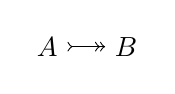
\begin{tikzpicture}[auto]
  \node (a) at (0, 0) {$A$};
  \node (b) at (1, 0) {$B$};
  \draw [>->>] (a) to node {} (b);
  \end{tikzpicture} } } $などと書く\footnote{圏論でいえばその記号は双射である、即ち、逆写像をもつような写像であることを意味してて写像であれば全単射ならそのときにかぎり逆写像をもつといえますが、圏論で扱う射では必ずしもそうとはいえなく全単射だからその記号がいつでも使えるというわけではないことに注意するといいかと思います。}。
\end{dfn}
\begin{thm}
\label{1.2.3.10}
写像$f:A \rightarrow B$について、次のことは同値である。
\begin{itemize}
\item
  その写像$f$は全単射である。
\item
  $\forall b \in B\exists!a \in A$に対し、$f(a) = b$が成り立つ。
\item
  写像$f:A \rightarrow B$の値域$V(f)$について、$V(f) = B$が成り立つかつ、$\forall f(a),f(b) \in B$に対し、$f(a) = f(b)$が成り立つなら、$a = b$が成り立つ。
\item
  $\forall b \in B\exists a \in A$に対し、$V\left( f^{- 1}|\left\{ b \right\} \right) = \left\{ a \right\}$が成り立つ。
\end{itemize}
\end{thm}
\begin{proof}
全単射な写像$f:A\overset{\sim}{\rightarrow}B$が与えられたとする。このとき、その写像$f$は全射でもあるので、$\forall b \in B\exists a \in A$に対し、$f(a) = b$が成り立つ。ここで、このような2つの元々$a$、$a'$がとられ$a \neq a'$が成り立つと仮定すると、その写像$f$は単射でもあるので、$f(a) = f\left( a' \right)$が成り立つ。これは仮定の$f(a) = f\left( a' \right) = b$に矛盾する。したがって、$\forall b \in B\exists!a \in A$に対し、$f(a) = b$が成り立つ。\par
逆に、これが成り立つなら、$\forall b \in B\exists a \in A$に対し、$f(a) = b$が成り立つので、その写像$f$は全射である。したがって、$B = V(f)$が成り立つ。さらに、$\forall b \in V(f) = B$に対し、明らかに$b \in V\left( f|\left\{ a \right\} \right)$が成り立つので、$a \in V\left( f^{- 1}|\left\{ b \right\} \right)$も成り立つ。ここで、仮定よりこのような元$a$はただ1つ存在するのであったので、$V\left( f^{- 1}|\left\{ b \right\} \right) = \left\{ a \right\}$が成り立つ。その写像$f$は単射でもあり、したがって、その写像$f$は全単射である。\par
その写像$f$が全単射であるなら、その写像$f$は単射でもあるので、$\forall f(a),f(b) \in B$に対し、$f(a) = f(b)$が成り立つなら、$a = b$が成り立つ。さらに、その写像$f$は全射であるので、$V(f) = B$が成り立つ。したがって、$V(f) = B$が成り立つかつ、$\forall f(a),f(b) \in B$に対し、$f(a) = f(b)$が成り立つなら、$a = b$が成り立つ。\par
逆に、これが成り立つなら、$V(f) = B$が成り立つので、その写像$f$は全射である。ここで、$\forall f(a),f(b) \in B$に対し、$f(a) = f(b)$が成り立つなら、$a = b$が成り立つので、その写像$f$は単射である。したがって、その写像$f$は全単射である。\par
また、その写像$f$が全単射であるなら、その写像$f$は単射でもあるので、$\forall b \in V(f)\exists a \in A$に対し、$V\left( f^{- 1}|\left\{ b \right\} \right) = \left\{ a \right\}$が成り立つ。さらに、その写像$f$は全射でもあり$V(f) = B$が成り立つので、$\forall b \in B\exists a \in A$に対し、$V\left( f^{- 1}|\left\{ b \right\} \right) = \left\{ a \right\}$が成り立つ。\par
逆に、これが成り立つなら、$V(f) \subseteq B$が成り立つので、その写像$f$は単射である。さらに、次のようになるので、
\begin{align*}
V\left( f|\left\{ a \right\} \right) = V\left( f|V\left( f^{- 1}|\left\{ b \right\} \right) \right) \subseteq \left\{ b \right\}
\end{align*}
$\forall b \in B\exists a \in A$に対し、$f(a) = b$が成り立ち、したがって、その写像$f$は全射である。以上より、その写像$f$は全単射である。
\end{proof}
%\hypertarget{ux6a19ux6e96ux7684ux5358ux5c04}{%
\subsubsection{標準的単射}%\label{ux6a19ux6e96ux7684ux5358ux5c04}}
\begin{thm}
\label{1.2.3.11}
集合$A$が与えられたとき、$\forall A'\in \mathfrak{P}(A)$に対し、次式のような写像$i$が考えられる。
\begin{align*}
i:A' \rightarrow A;a \mapsto a
\end{align*}
これについて、次のことが成り立つ。
\begin{itemize}
\item
  その写像$i$は単射である。
\item
  その写像$i$の値域$V(i)$について、$V(i) = A'$が成り立つ。
\item
  $A' = A$が成り立つなら、その写像$i$は全単射となる。
\end{itemize}
\end{thm}
\begin{dfn}
このような写像$i$を特にその集合$A'$からその集合$A$への標準的単射、自然な単射、包含写像などといい$A' \hookrightarrow A$などと書く。
\end{dfn}
\begin{proof}
集合$A$が与えられたとき、$\forall A'\in \mathfrak{P}(A)$に対し、次式のような写像$i$が考えられる。
\begin{align*}
i:A' \rightarrow A;a \mapsto a
\end{align*}
ここで、$\forall a,b \in A'$に対し、$a \neq b$が成り立つなら、$i(a) = a$かつ$i(b) = b$が成り立つので、$i(a) \neq i(b)$が成り立つ。これにより、その写像$i$は単射となる。\par
また、その写像$i$の値域$V(i)$について、$V(i) = \bigcup_{a \in A'} {V\left( i|\left\{ a \right\} \right)}$が成り立つのであった。したがって、その対応$i$が写像であるので、$V\left( i|\left\{ a \right\} \right) = \left\{ i(a) \right\}$が成り立つことに注意すれば、次式のようになる。
\begin{align*}
V(i) = \bigcup_{a \in A'} {V\left( i|\left\{ a \right\} \right)} = \bigcup_{a \in A'} \left\{ i(a) \right\} = \bigcup_{a \in A'} \left\{ a \right\} = A'
\end{align*}\par
$A' = A$が成り立つなら、上記の議論により$V(i) = A' = A$が成り立つので、定義より明らかにその写像$i$は全射である。したがって、その写像$i$は全単射となる。
\end{proof}
%\hypertarget{ux9006ux5199ux50cf}{%
\subsubsection{逆写像}%\label{ux9006ux5199ux50cf}}
\begin{dfn}
写像$f$の逆対応$f^{- 1}$は必ずしも写像になるとは限らないが、写像になるときがありこの写像$f^{- 1}$をその写像$f$の逆写像という。
\end{dfn}
\begin{thm}
\label{1.2.3.12}
写像$f$が全単射であるならそのときに限り、その写像$f$の逆写像$f^{- 1}$が存在する。
\end{thm}
\begin{proof}
写像$f:A \rightarrow B$が全単射であるならそのときに限り、定理\ref{1.2.3.10}より$\forall b \in B\exists a \in A$に対し、$V\left( f^{- 1} \middle| \left\{ b \right\} \right) = \left\{ a \right\}$が成り立つ。これが成り立つならそのときに限り、その逆対応$f^{- 1}$は写像となっているので、その写像$f$の逆写像$f^{- 1}$が存在する。\par
逆に、写像$f$の逆写像$f^{- 1}$が存在するなら、$\forall b \in B\exists a \in A$に対し、$V\left( f^{- 1} \middle| \left\{ b \right\} \right) = \left\{ a \right\}$が成り立つので、これが成り立つならそのときに限り、定理\ref{1.2.3.10}よりその写像$f$は全単射である。
\end{proof}
\begin{thm}
\label{1.2.3.13}
写像$f$の逆写像$f^{- 1}$が存在すれば、これは必ず全単射となる。
\end{thm}
\begin{proof}
写像$f$の逆写像$f^{- 1}$が存在すれば、これの逆対応$\left( f^{- 1} \right)^{- 1}$が考えられると、$\left( f^{- 1} \right)^{- 1} = f$が成り立つのであったので、その逆対応$\left( f^{- 1} \right)^{- 1}$も写像となっている。定理\ref{1.2.3.12}より、その写像$f^{- 1}$は全単射である。
\end{proof}
%\hypertarget{ux5408ux6210ux5199ux50cf}{%
\subsubsection{合成写像}%\label{ux5408ux6210ux5199ux50cf}}
\begin{dfn}
2つの写像たち$f:A \rightarrow B$、$g:B \rightarrow C$が与えられたとする。このとき、$V(f) \subseteq D(g)$が成り立つとき、次式のような写像$\varphi$が存在する。この写像$\varphi$をその写像$f$とその写像$g$の合成写像といい$g \circ f$と書く。
\begin{align*}
g \circ f:A \rightarrow C;a \mapsto g\left( f(a) \right)
\end{align*}
\end{dfn}
このとき、必ずしも$g \circ f = f \circ g$が成り立つとは限らないことに注意されたい\footnote{例えば、定値写像$\hat{a} :\{a,b\}\rightarrow \{a,b\} ;x\mapsto a$、$\hat{b} :\{a,b\}\rightarrow \{a,b\} ;x\mapsto b$が挙げられ、実際、$\hat{a} \circ \hat{b} \ne \hat{b} \circ \hat{a} $が成り立つ。}。
\begin{thm}
\label{1.2.3.14}
次のことが成り立つ。
\begin{itemize}
\item
  2つの写像たち$f:A \rightarrow B$、$g:B \rightarrow C$がどちらも全射であるとき、その合成写像$g \circ f$も全射である。
\item
  2つの写像たち$f:A \rightarrow B$、$g:B \rightarrow C$がどちらも単射であるとき、その合成写像$g \circ f$も単射である。
\item
  2つの写像たち$f:A \rightarrow B$、$g:B \rightarrow C$がどちらも全単射であるとき、その合成写像$g \circ f$も全単射である。
\end{itemize}
\end{thm}
\begin{proof}
2つの写像たち$f:A \rightarrow B$、$g:B \rightarrow C$がどちらも全射であるとき、$\forall c \in C\exists b \in B$に対し、$c = g(b)$が成り立ち、さらに、$\exists a \in A$に対し、$b = f(a)$が成り立つので、$c = g\left( f(a) \right)$が成り立つ。これにより、その写像$g \circ f$は全射となる。\par
2つの写像たち$f:A \rightarrow B$、$g:B \rightarrow C$がどちらも単射であるとき、$\forall a,b \in A$に対し、$a \neq b$が成り立つなら、$f(a) \neq f(b)$が成り立ち、$g\left( f(a) \right) \neq g\left( f(b) \right)$が成り立つ。これにより、その写像$g \circ f$は単射となる。\par
定義より2つの写像たち$f:A \rightarrow B$、$g:B \rightarrow C$がどちらも全単射であるとき、2つの写像たち$f:A \rightarrow B$、$g:B \rightarrow C$がどちらも全射であるかつ、単射であるので、上記の議論によりその合成写像$g \circ f$も全射であるかつ、単射であるので、その合成写像$g \circ f$も全単射となる。
\end{proof}
\begin{thm}
\label{1.2.3.15}
次のことも成り立つ。
\begin{itemize}
\item
  2つの写像たち$f:A \rightarrow B$、$g:B \rightarrow C$の合成写像$g \circ f$が全射であるとき、その写像$g$も全射である。
\item
  2つの写像たち$f:A \rightarrow B$、$g:B \rightarrow C$の合成写像$g \circ f$が単射であるとき、その写像$f$も単射である。
\end{itemize}
\end{thm}
\begin{proof}
2つの写像たち$f:A \rightarrow B$、$g:B \rightarrow C$の合成写像$g \circ f$が全射であるならそのときに限り、$\forall c \in C\exists a \in A$に対し、$c = g \circ f(a)$が成り立つ。ここで、$f(a) = b$とおくと、その対応$f$は写像であるので、そのような元$b$は存在し、次式が成り立つ。
\begin{align*}
c = g \circ f(a) = g\left( f(a) \right) = g(b)
\end{align*}
これが成り立つならそのときに限り、その写像$g$は全射である。\par
2つの写像たち$f:A \rightarrow B$、$g:B \rightarrow C$の合成写像$g \circ f$が単射であるとき、$\forall a,b \in A$に対し、$a \neq b$が成り立つとき、$g \circ f(a) \neq g \circ f(b)$が成り立つ。このとき、$g \circ f(a) \neq g \circ f(b)$が成り立つかつ、$f(a) = f(b)$が成り立つとすると、次のようになり
\begin{align*}
g \circ f(a) = g\left( f(a) \right) = g\left( f(b) \right) = g \circ f(b)
\end{align*}
これは$g \circ f(a) \neq g \circ f(b)$が成り立つことに矛盾する。したがって、$g \circ f(a) \neq g \circ f(b)$が成り立つなら、$f(a) \neq f(b)$が成り立つ。以上より、その写像$f$は単射となる。
\end{proof}
\begin{thm}
\label{1.2.3.16}
また、合成写像の性質として次のことが成り立つ。
\begin{itemize}
\item
  3つの写像たち$f:A \rightarrow B$、$g:B \rightarrow C$、$h:C \rightarrow D$が与えられたとき、$h \circ (g \circ f) = (h \circ g) \circ f$が成り立つ。
\item
  写像$f:A \rightarrow B$が与えられたとき、$f \circ I_{A} = I_{B} \circ f = f$が成り立つ。
\item
  写像たち$f:A \rightarrow B$、$g:B \rightarrow A$が与えられたとき、それらの写像たちどちらも全単射で$g = f^{- 1}$が成り立つならそのときに限り、$g \circ f = I_{A}$かつ$f \circ g = I_{B}$が成り立つ。
\item
  写像たち$f:A \rightarrow B$、$g:B \rightarrow C$が与えられたとき、それらの写像たちどちらも全単射であるなら、$(g \circ f)^{- 1} = f^{- 1} \circ g^{- 1}$が成り立つ。
\end{itemize}
\end{thm}
\begin{proof}
3つの写像たち$f:A \rightarrow B$、$g:B \rightarrow C$、$h:C \rightarrow D$が与えられたとき、$\forall a \in A$に対し、次のようになるので、
\begin{align*}
h \circ (g \circ f)(a) = h\left( g \circ f(a) \right) = h\left( g\left( f(a) \right) \right) = h \circ g\left( f(a) \right) = (h \circ g) \circ f(a)
\end{align*}
したがって、$h \circ (g \circ f) = (h \circ g) \circ f$が成り立つ。\par
写像$f:A \rightarrow B$が与えられたとき、$\forall a \in A$に対し、次のようになる。
\begin{align*}
f \circ I_{A}(a) &= f\left( I_{A}(a) \right) = f(a)\\
I_{B} \circ f(a) &= I_{B}\left( f(a) \right) = f(a)
\end{align*}
したがって、$f \circ I_{A} = I_{B} \circ f = f$が成り立つ。\par
写像たち$f:A \rightarrow B$、$g:B \rightarrow A$が与えられたとき、それらの写像たちどちらも全単射で$g = f^{- 1}$が成り立つなら、$\forall a \in A$に対し、次式が成り立つかつ、
\begin{align*}
g \circ f(a) = f^{- 1} \circ f(a) = f^{- 1}\left( f(a) \right) = a = I_{A}(a)
\end{align*}
$\forall b \in B$に対し、次式が成り立つので、
\begin{align*}
f \circ g(a) = f \circ f^{- 1}(b) = f\left( f^{- 1}(b) \right) = b = I_{B}(b)
\end{align*}
$g \circ f = I_{A}$かつ$f \circ g = I_{B}$が成り立つ。\par
逆に、$g \circ f = I_{A}$かつ$f \circ g = I_{B}$が成り立つなら、その写像$I_{A}$は全単射であるので、その写像$g$は全射でその写像$f$は単射である。同様にして、その写像$I_{B}$は全単射であるので、その写像$f$は全射でその写像$g$は単射である。以上より、それらの写像たち$f$、$g$はどちらも全単射となる。また、上記の議論により次のようになるので、
\begin{align*}
g = g \circ I_{B} = g \circ \left( f \circ f^{- 1} \right) = (g \circ f) \circ f^{- 1} = I_{A} \circ f^{- 1} = f^{- 1}
\end{align*}
$g = f^{- 1}$が成り立つ。\par
写像たち$f:A \rightarrow B$、$g:B \rightarrow C$が与えられたとき、それらの写像たちどちらも全単射であるなら、その合成写像$g \circ f$も全単射となるので、その合成写像$g \circ f$の逆写像$(g \circ f)^{- 1}$が存在する。このとき、写像$f^{- 1} \circ g^{- 1}$について次式が成り立つので、
\begin{align*}
\left( f^{- 1} \circ g^{- 1} \right) \circ (g \circ f) &= f^{- 1} \circ \left( g^{- 1} \circ g \right) \circ f = f^{- 1} \circ I_{B} \circ f = f^{- 1} \circ f = I_{A}\\
(g \circ f) \circ \left( f^{- 1} \circ g^{- 1} \right) &= g \circ \left( f \circ f^{- 1} \right) \circ g^{- 1} = g \circ I_{B} \circ g^{- 1} = g \circ g^{- 1} = I_{C}
\end{align*}
$(g \circ f)^{- 1} = f^{- 1} \circ g^{- 1}$が成り立つ。
\end{proof}
%\hypertarget{ux5199ux50cfux306eux59cbux96c6ux5408ux3068ux7d42ux96c6ux5408}{%
\subsubsection{写像の始集合と終集合}%\label{ux5199ux50cfux306eux59cbux96c6ux5408ux3068ux7d42ux96c6ux5408}}
\begin{dfn}
写像$f:A \rightarrow B$が与えられたとき、$\forall A'\in \mathfrak{P}(A)$に対し、次式のような写像$f'$が定義される。この写像$f'$も対応と同じくその写像$f$の始集合$A$をその集合$A'$に縮小された、制限された写像などといい$f|A'$、$\left. f \right|_{A'} $などと書く。
\begin{align*}
f':A' \rightarrow B;a \mapsto f(a)
\end{align*}
逆に、その写像$f$はその写像$f|A'$の始集合$A'$をその集合$A$に拡大された、延長された写像などという。
\end{dfn}
\begin{thm}
\label{1.2.3.17}
その写像$f$とその集合$A'$が与えられたとき、その写像$f|A'$は一意的に存在する。\par
\end{thm}
逆に、その写像$f|A'$とその集合$A$が与えられたときでもその写像$f|A'$の始集合$A'$をその集合$A$に拡大された写像は一意的であるとは限らないことに注意されたい。
\begin{proof}
その写像$f$とその集合$A'$が与えられたとき、定義より明らかにその写像$f|A'$は存在する。ここで、次式のような写像たち$f'$、$f''$が与えられたとする。
\begin{align*}
f':A' \rightarrow B;a \mapsto f(a),\ \ f'':A' \rightarrow B;a \mapsto f(a)
\end{align*}
このとき、$\forall a \in A'$に対し、次式が成り立つので、
\begin{align*}
f'(a) = f(a) = f''(a)
\end{align*}
$f' = f''$が成り立つ。
\end{proof}
対応の定義より明らかであるように、写像$f:A \rightarrow B$の終集合$B$がこの集合$B$とは異なる集合$B'$に変えられたときの写像はもとのその写像$f$とは異なるものとみなされる。ただ、その集合$B'$が$V(f) \subseteq B'$を満たすとき、その終集合$B$がこの集合$B$とは異なる集合$B'$に変えられたときの写像はもとのその写像$f$と同じものとみなされるときがあることに注意されたい。
\subsubsection{集合族}
\begin{dfn}
空でない集合$\varLambda$と集合$A$を用いて、写像$a:\varLambda \rightarrow A$を考えるとき、順序対$\left( a,V(a) \right)$をその集合$\varLambda$によって添数づけられた集合といい、その集合$\varLambda$をその集合$\left( a,V(a) \right)$の添数集合、これの元$\lambda$を添数という。ここで、$a(\lambda)$を$a_{\lambda}$とも書き、その値域$V(a)$は定義より$\left\{ a' \in A \middle| \exists\lambda \in \varLambda\left[ a' = a(\lambda) \right] \right\}$とも書かれることができ、分出の公理と存在除去より直ちに$\left\{ a_{\lambda} \in A \middle| \lambda \in \varLambda \right\}$とも書かれることができる。これをその添数集合$\varLambda$によって添数づけられたその集合$A$の集合族、元の族などといい単に$\left\{ a_{\lambda} \middle| \lambda \in \varLambda \right\}$、$\left\{ a_{\lambda} \right\}_{\lambda \in \varLambda}$などとも書く。さらに、その写像$a$をその集合$A$のその添数集合$\varLambda$によって順序づけられた組などといい次式のように$\left( a_{\lambda} \right)_{\lambda \in \varLambda}$、$\left( a_{\lambda} \in A \middle| \lambda \in \varLambda \right)$などとも書く。
\begin{center}
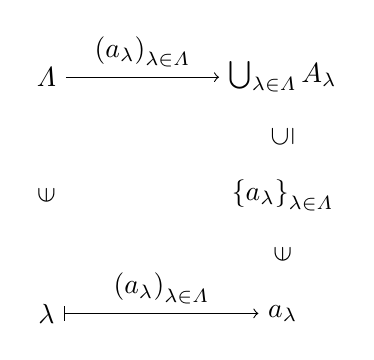
\begin{tikzpicture}[auto] 

  \node (e) at (0, 0) {$\lambda $};
  \node (f) at (3, 0) {$a_{\lambda } $};
  \node (g) at (0, 3) {$\varLambda $};
  \node (h) at (3, 3) {$\bigcup_{\lambda \in \varLambda } A_{\lambda } $};
  \node[rotate=90] (m) at (0, 1.5) {$\in $};
  \node[rotate=90] (m) at (3, 0.75) {$\in $};
  \node (n) at (3, 1.5) {$\left\{ a_{\lambda } \right\}_{\lambda \in \varLambda } $};
  \node[rotate=90] (o) at (3, 2.25) {$\subseteq $};
  \draw [|->] (e) to node {$\left( a_{\lambda } \right)_{\lambda \in \varLambda } $} (f);
  \draw [->] (g) to node {$\left( a_{\lambda } \right)_{\lambda \in \varLambda } $} (h);

\end{tikzpicture}
\end{center}
\end{dfn}
\begin{dfn}
次式で定義される集合$\prod_{\lambda \in \varLambda} A_{\lambda}$を空でない集合$\varLambda$によって添数づけられた集合$\left\{ A_{\lambda} \right\}_{\lambda \in \varLambda}$の一般化された直積という。なお、集合$\mathfrak{F}\left( \varLambda,\bigcup_{\lambda \in \varLambda} A_{\lambda} \right)$に属し、$\forall\lambda \in \varLambda$に対し、$f(\lambda) \in A_{\lambda}$なる写像$f$を用いた集合$f(\lambda)$を$a_{\lambda}$とおいた。
\begin{align*}
\prod_{\lambda \in \varLambda} A_{\lambda} = \left\{ f \in \mathfrak{F}\left( \varLambda,\bigcup_{\lambda \in \varLambda} A_{\lambda} \right) \middle| \forall\lambda \in \varLambda\left[ f(\lambda) \in A_{\lambda} \right] \right\}
\end{align*}
その写像$f$は次式のようにも書かれることができる。
\begin{center}
\begin{tikzpicture}[auto] 
  
  \node (i) at (0, 0) {$\lambda $};
  \node (j) at (3, 0) {$f \left( \lambda \right) $};
  \node (k) at (0, 3) {$\varLambda $};
  \node (l) at (3, 3) {$\bigcup_{\lambda \in \varLambda } A_{\lambda } $};
  \node[rotate=90] (m) at (0, 1.5) {$\in $};
  \node[rotate=90] (m) at (3, 0.75) {$\in $};
  \node[rotate=90] (o) at (3, 2.25) {$\subseteq $};
  \node (p) at (3, 1.5) {$A_{\lambda } $};
  \draw [|->] (i) to node {$f$} (j);
  \draw [->] (k) to node {$f$} (l);
  
\end{tikzpicture}
\end{center}
\end{dfn}
このとき、$f \in \prod_{\lambda \in \varLambda} A_{\lambda}$が成り立つならそのときに限り、写像$f:\varLambda \rightarrow \bigcup_{\lambda \in \varLambda} A_{\lambda}$が与えられ、$\forall\lambda \in \varLambda$に対し、$f(\lambda) \in A_{\lambda}$が成り立つのであった。これにより、その写像$f$はその集合$\bigcup_{\lambda \in \varLambda} A_{\lambda}$のその添数集合$\varLambda$によって順序づけられた組となっている。
\begin{dfn}
特に、集合$A$が与えられたとき、添数集合$\varLambda$によって添数づけられたその集合$\mathfrak{P}(A)$の集合族$\left\{ a_{\lambda} \right\}_{\lambda \in \varLambda}$をその集合$A$の部分集合族などという。もちろん、$\varLambda = \mathbb{N}$が成り立つなら、その集合$A$の写像$\left( a_{\lambda} \right)_{\lambda \in \varLambda}$はその集合$A$の無限列であるし、$\varLambda = \varLambda_{n}$が成り立つなら、その集合$A$の写像$\left( a_{\lambda} \right)_{\lambda \in \varLambda}$はその集合$A$の長さが$n$の有限列である。
\end{dfn}
\begin{dfn}
添数$\lambda$に依存しない集合$A$を用いた直積$\prod_{\lambda \in \varLambda_{n}} A$を$A^{n}$と書くことがある。
\end{dfn}
\begin{thm}\label{1.2.5.3}
添数集合$\varLambda$を用いた空集合でない直積$\prod_{\lambda \in \varLambda} A_{\lambda}$について、次式のような写像${\mathrm{pr}}_{\lambda}$が定義されるとき、
\begin{center}
\begin{tikzpicture}[auto] 

  \node (a) at (0, 0) {$\left( a_{\lambda } \right)_{\lambda \in \varLambda } $};
  \node (b) at (3, 0) {$a_{\lambda } $};
  \node (c) at (0, 3) {$\prod_{\lambda \in \varLambda } A_{\lambda } $};
  \node (d) at (3, 3) {$A_{\lambda } $};
  \node[rotate=90] (m) at (0, 1.5) {$\in $};
  \node[rotate=90] (m) at (3, 1.5) {$\in $};
  \draw [|->] (a) to node {${\rm pr}_{\lambda } $} (b);
  \draw [->] (c) to node {${\rm pr}_{\lambda } $} (d);

\end{tikzpicture}
\end{center}
このような写像${\mathrm{pr}}_{\lambda}$は存在する。
\end{thm}
\begin{proof}
添数集合$\varLambda$を用いた空集合でない直積$\prod_{\lambda \in \varLambda} A_{\lambda}$について、次式のような写像${\mathrm{pr}}_{\lambda'}$が定義されるとき、
\begin{align*}
{\mathrm{pr}}_{\lambda}:\prod_{\lambda \in \varLambda} A_{\lambda} \rightarrow A_{\lambda};\left( a_{\lambda} \right)_{\lambda \in \varLambda} \mapsto a_{\lambda}
\end{align*}
その直積$\prod_{\lambda \in \varLambda} A_{\lambda}$は空集合ではないので、$\forall\lambda \in \varLambda$に対し$A_{\lambda} \neq \emptyset$が成り立ち、したがって、$\forall\left( a_{\lambda} \right)_{\lambda \in \varLambda} \in \prod_{\lambda \in \varLambda} A_{\lambda}$に対し、その元$a_{\lambda}$がその集合$A_{\lambda}$に存在する。また、定義より明らかにその元$a_{\lambda}$は一意的である。
\end{proof}
\begin{dfn}
このような写像${\mathrm{pr}}_{\lambda}$をその直積$\prod_{\lambda \in \varLambda} A_{\lambda}$からその集合$A_{\lambda}$へのその添数$\lambda$における射影といい$\mathrm{proj}_{\lambda}$ともかく\footnote{ああいうminorだけど便利なヤツたまにあるんだよね(*`∀`)}。さらにここでは、記法上の都合上、$\mathrm{pr}_\lambda $をさらに$1_\lambda $とも書くことにする\footnote{ローカルルール注意です...。}。
\end{dfn}
\begin{dfn}
さらに、その添数$\lambda$における射影${\mathrm{pr}}_{\lambda}$によるその添数づけられたその集合$\bigcup_{\lambda \in \varLambda} A_{\lambda}$の集合族$\left\{ a_{\lambda} \right\}_{\lambda \in \varLambda}$の像$a_{\lambda}$をその順序づけられた組$\left( a_{\lambda} \right)_{\lambda \in \varLambda}$の$\lambda$成分、$\lambda$座標などという。
\end{dfn}
\subsubsection{$n$項演算}
\begin{dfn}
次式のように直積$\prod_{\lambda \in \varLambda} A_{\lambda}$から集合$B$への写像$f$が与えられたとする。
\begin{align*}
f:\prod_{\lambda \in \varLambda} A_{\lambda} \rightarrow B
\end{align*}
このとき、その直積$\prod_{\lambda \in \varLambda} A_{\lambda}$の任意の元は順序づけられた組$\left( a_{\lambda} \right)_{\lambda \in \varLambda}$となっているので、これのその写像$f$による像$f\left( \left( a_{\lambda} \right)_{\lambda \in \varLambda} \right)$を単に$f\left( a_{\lambda} \right)_{\lambda \in \varLambda}$と書く。
\end{dfn}
\begin{dfn}
ある集合たち$A$、$B$を用いた次式のような写像$f$が与えられたとき、その写像$f$は$n$項演算などという。
\begin{align*}
f:\prod_{\lambda \in \varLambda_{n}} A \rightarrow B
\end{align*}
特に、$n = 2$とした$n$項演算を単に演算、算法などという。
\end{dfn}
\begin{dfn}
さらに、誤解の恐れがないとき、写像$\rho :\prod_{\lambda \in \Lambda } B_{\lambda } \rightarrow V$と写像の族$\{f_{\lambda } :A_{\lambda } \rightarrow B_{\lambda } \}_{\lambda \in \varLambda }$が与えられたとき、次のように定義される写像$f$を$\rho \left(f_{\lambda } \right)_{\lambda \in \varLambda }$と略記する。
\begin{align*}
f:\prod_{\lambda \in \Lambda } A_{\lambda } \rightarrow V;\left( a_{\lambda } \right)_{\lambda \in \varLambda } \mapsto \rho \left(f_{\lambda } \left(a_{\lambda } \right) \right)_{\lambda \in \varLambda }
\end{align*}
\end{dfn}
\subsubsection{写像に関する一定理}
\begin{thm}\label{1.2.5.4}
写像$f:A \rightarrow B$において、次のことが成り立つ。
\begin{itemize}
\item
  その写像$f$が全射であるならそのときに限り、$f \circ g = I_{B}$が成り立つような写像$g:B \rightarrow A$が存在する。
\item
  その写像$f$が単射であるならそのときに限り、$g \circ f = I_{A}$が成り立つような写像$g:B \rightarrow A$が存在する。
\end{itemize}
\end{thm}
\begin{proof} 写像$f:A \rightarrow B$が与えられたとする。\par
$f \circ g = I_{B}$が成り立つような写像$g:B \rightarrow A$が存在するかつ、その写像$f$が全射でないと仮定しよう。このとき、$V(f) \subset B$が成り立つので、$b \in V(f) \setminus B$なる元$b$について、恒等写像の定義より$f \circ g(b) = I_{B}(b) = b \in V(f) \setminus B$が成り立つ。一方で、その対応$g$は写像であったので、$D(g) = B$が成り立ち、したがって、$g(b) \in A$が成り立つ。これにより、$f\left( g(b) \right) = f \circ g(b) \in V(f)$が成り立つことになるが、これは$f \circ g(b) \in V(f) \setminus B$が成り立つことに矛盾する。したがって、$f \circ g = I_{B}$が成り立つような写像$g:B \rightarrow A$が存在するなら、その写像$f$が全射である。\par
逆に、その写像$f$が全射であるとき、$V(f) = B$が成り立つので、$\forall b \in B$に対しその写像$f$のgraph$G$を用いて$(a,b) \in G$となる元$a$が存在する。したがって、$V\left( f^{- 1}|\left\{ b \right\} \right)$は空集合ではない。ここで、選択の公理よりその集合族$\left\{ V\left( f^{- 1}|\left\{ b \right\} \right) \right\}_{b \in B}$の選択写像を$c$とすれば、$V\left( f^{- 1}|\left\{ b \right\} \right)$は空集合ではないので、$c\left( V\left( f^{- 1}|\left\{ b \right\} \right) \right) \in V\left( f^{- 1}|\left\{ b \right\} \right)$が成り立つ。ここで、次式のような写像$g$を考えると、
\begin{align*}
g:B \rightarrow A;b \mapsto c\left( V\left( f^{- 1}|\left\{ b \right\} \right) \right)
\end{align*}
$\forall b \in B$に対し、$g(b) \in V\left( f^{- 1}|\left\{ b \right\} \right)$が成り立つので、$\left( g(b),b \right) \in G$が成り立ち$b \in V\left( f|\left\{ g(b) \right\} \right)$が成り立つ。ここで、その対応$f$は写像であったので、$V\left( f|\left\{ g(b) \right\} \right) = \left\{ b \right\}$が成り立ち、したがって、$f \circ g(b) = f\left( g(b) \right) = b = I_{B}(b)$が成り立つ。以上より、$\forall b \in B$に対し、$f \circ g(b) = I_{B}(b)$が成り立つので、$f \circ g = I_{B}$が成り立つような写像$g:B \rightarrow A$が存在する。\par
よって、その写像$f$が全射であるならそのときに限り、$f \circ g = I_{B}$が成り立つような写像$g:B \rightarrow A$が存在する。\par
$g \circ f = I_{A}$が成り立つような写像$g:B \rightarrow A$が存在するかつ、その写像$f$は単射でないと仮定しよう。このとき、$a \neq b$かつ$f(a) = f(b)$が成り立つような元々$a$、$b$がその集合$A$に存在することになる。したがって、恒等写像の定義より$g \circ f(a) = I_{A}(a) = a$かつ$g \circ f(b) = I_{A}(b) = b$が成り立つので、$g \circ f(a) \neq g \circ f(b)$が成り立つ。一方で、次式が成り立つが、
\begin{align*}
g \circ f(a) = g\left( f(a) \right) = g\left( f(b) \right) = g \circ f(b)
\end{align*}
これは$g \circ f(a) \neq g \circ f(b)$が成り立つことに矛盾する。したがって、次式が成り立つような写像$g:B \rightarrow A$が存在するなら、
\begin{align*}
g \circ f = I_{A}
\end{align*}
その写像$f$は単射である。\par
逆に、その写像$f$が単射であるとき、次式のような写像$f'$を考えると、
\begin{align*}
f':A \rightarrow V(f);a \mapsto f(a)
\end{align*}
その写像$f'$は全単射である。したがって、その写像$f'$の逆対応${f'}^{- 1}$は写像になる。ここで、$\forall a' \in A$に対し、次式のように写像$g$を定めると、
\begin{align*}
g:B \rightarrow A;b \mapsto \left\{ \begin{matrix}
{f'}^{- 1}(b) & {\mathrm{if}} & b \in V(f) \\
a' & {\mathrm{if}} & b \notin V(f) \\
\end{matrix} \right.\ 
\end{align*}
$\forall a \in A$に対し、$f(a) = f'(a) \in V(f)$が成り立つことに注意すれば、次のようになる。
\begin{align*}
g \circ f(a) = g\left( f(a) \right) = g\left( f'(a) \right) = {f'}^{- 1}\left( f'(a) \right) = {f'}^{- 1} \circ f'(a) = I_{A}(a) = a
\end{align*}
したがって、$g \circ f = I_{A}$が成り立つような写像$g:B \rightarrow A$が存在する。\par
よって、その写像$f$が単射であるならそのときに限り、$g \circ f = I_{A}$が成り立つような写像$g:B \rightarrow A$が存在する。
\end{proof}
\begin{thm}\label{1.2.5.5}
2つの集合たち$A$、$B$が与えられたとする。その集合$Aからその集合B$への単射が存在するならそのときに限り、その集合$Bからその集合A$への全射が存在する。
\end{thm}
\begin{proof}
2つの集合たち$A$、$B$が与えられたとする。単射$f:A \rightarrowtail B$が存在すらそのときに限り$g \circ f = I_{A}$が成り立つような写像$g:B \rightarrow A$が存在する。このような写像$f:A \rightarrow B$が存在するならそのときに限り、全射$g:B \twoheadrightarrow A$が存在する。
\end{proof}
\begin{thebibliography}{50}
  \bibitem{1}
    Rei Frontier Tech Blog. "ZFC公理系について:その1". Hatena Blog. \url{https://tech-blog.rei-frontier.jp/entry/2017/11/02/102042}, (2021-04-01 20:30 閲覧)
  \bibitem{2}
    Rei Frontier Tech Blog. "ZFC公理系について:その2". Hatena Blog. \url{https://tech-blog.rei-frontier.jp/entry/2017/11/09/100000}, (2021-04-01 20:30 閲覧)
  \bibitem{3}
    Rei Frontier Tech Blog. "ZFC公理系について:その3". Hatena Blog. \url{https://tech-blog.rei-frontier.jp/entry/2017/11/16/100000} (2021-04-01 20:30 閲覧)
  \bibitem{4}
    松坂和夫, 集合・位相入門, 岩波書店, 1968. 新装版第2刷 p39 ISBM978-4-00-029871-1
  \bibitem{5}
    WIIS. "写像による逆像". WIIS. \url{https://wiis.info/math/set/mapping/mapping-inverse-image/} (2021-2-27 15:30 閲覧)
  \bibitem{6}
    尾畑伸明. "第4章 写 像". 東北大学. \url{https://www.math.is.tohoku.ac.jp/~obata/student/subject/file/2018-4_shazo.pdf} (2021-2-27 15:45 閲覧)
\end{thebibliography}
\end{document}
